\setcounter{chapter}{9}
\chapter{Radon Transform}
\pgr{VisComp07a_Radon}{19}{-1.7}{-1.45}{1.8}{0.9}
\begin{center}
		\def\rsize{0.7}
		\def\hrsize{0.5*\rsize}
		\def\phsize{1.5*\rsize}
	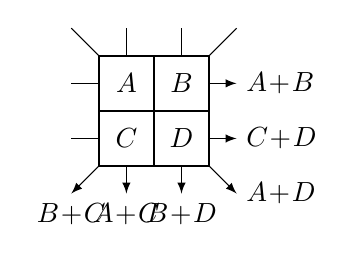
\begin{tikzpicture}[radon rectangle/.style={rectangle,fill=white,draw,thick,minimum width=\rsize cm,minimum height=\rsize cm}]
		\draw[-latex] (-\hrsize,\phsize) -- (-\hrsize,-\phsize) coordinate[label=below:$\miniscule A\!+\!C$] (ac);
		\draw[-latex] (\hrsize,\phsize) -- (\hrsize,-\phsize) coordinate[label=below:$\miniscule B\!+\!D$] (bd);
		\draw[-latex] (-\phsize,\hrsize) -- (\phsize,\hrsize) coordinate[label=right:$\miniscule A\!+\!B$] (ab);
		\draw[-latex] (-\phsize,-\hrsize) -- (\phsize,-\hrsize) coordinate[label=right:$\miniscule C\!+\!D$] (ab);
		\draw[-latex] (-\phsize,\phsize) -- (\phsize,-\phsize) coordinate[label=right:$\miniscule A\!+\!D$] (ad);
		\draw[-latex] (\phsize,\phsize) -- (-\phsize,-\phsize) coordinate[label=below:$\miniscule B\!+\!C$] (bc);
		\node[radon rectangle] (a) at (-\hrsize,\hrsize) {$A$};
		\node[radon rectangle] (b) at (\hrsize,\hrsize) {$B$};
		\node[radon rectangle] (c) at (-\hrsize,-\hrsize) {$C$};
		\node[radon rectangle] (d) at (\hrsize,-\hrsize) {$D$};
	\end{tikzpicture}
	\begin{align*}
		\left[
		\begin{smallmatrix}
			1&1&0&0\\
			1&0&1&0\\
			1&0&0&1\\
			0&1&1&0\\
			0&1&0&1\\
			0&0&1&1\\
			1&1&0&0\\
		\end{smallmatrix}
		\right]\!\!
		\left[
		\begin{smallmatrix}
			A\\
			B\\
			C\\
			D\\
		\end{smallmatrix}
		\right]
		&=
		\left[
		\begin{smallmatrix}
			A+B\\
			A+C\\
			A+D\\
			B+C\\
			B+D\\
			C+D\\
		\end{smallmatrix}
		\right]\\
		\Leftrightarrow K\vtr{x}&=\vtr{b}\\
		\leadsto K^TK\vtr{x}&=K^T\vtr{b}\\
		\leadsto{\!\left[ K^TK \right]\!}^{-1}K^{T}\vtr{b}&= \vtr{x}
	\end{align*}
\end{center}
Over-determined non-square matrix $K$. Larger problems must be solved iteratively using standard methods for solving large matrix operation problems.
\section{Definition}
\pgr{VisComp07a_Radon}{23}{0.6}{-1.1}{2.4}{0.9}
We will use teh coordinate system defined in the figure above to describe line integrals and projections. In this example the object is represented by a two-dimensional function $f(x,y)$ and each line integral by the $(\theta,t)$ parameters. The equation of line $AB$ in the figure above is
\begin{gather*}
	x\cos\theta+y\sin\theta=t
\end{gather*}
and we will use this relationship to define line integral $P_{\theta}$ as
\begin{gather*}
	P_{\theta}(t)={\scriptstyle\int_{(\theta,t)\text{line}}}^{}\!\dd{s}\, f(x,y)
\end{gather*}
Using a delta function, this can be rewritten as
\begin{align*}
	P_{\theta}(t)&={\scriptstyle\int_{\mathbb{R}^2}}\dd{x}\!\dd{y}\, f(x,y)\\
	&\hphantom{\int_{\mathbb{R}^2}\cdot}\cdot\delta(x\cos\theta+y\sin\theta-t)
\end{align*}
\section{Fourier Slice Theorem}
Two-dimensional Fourier transform of the object function
\begin{align*}
	F(u,v)&={\scriptstyle\int_{\mathbb{R}^2}^{}}\dd{x}\!\dd{y}\, f(x,y)\\
	&\hphantom{{\scriptstyle\int_{\mathbb{R}^2}^{}}\cdot}\cdot e^{-j2\pi(ux+vy)}
\end{align*}
Likewise, define a projection at an angle $\theta$, $P_{\theta}(t)$, and its fourier transform by 
\begin{gather*}
	S_{\theta}(w)={\scriptstyle\int_{\mathbb{R}^2}^{}}\dd{t}\, P_{\theta}(t)e^{-j2\pi wt}
\end{gather*}
The simplest example of the Fourier Slice Theorem is given for a projection at $\theta=0$. First, consider the Fourier transform of the object along the line in the frequency domain given by $v=0$. The Fourier transform integral now simplifies to $F(u,0)$
\begin{align*}
	&={\scriptstyle\int_{\mathbb{R}^2}^{}}\dd{x}\!\dd{y}\, f(x,y)e^{-j2\pi ux}\\
	&={\scriptstyle\int_{-\infty}^{\infty}}\dd{x}\, P_{\theta=0}e^{-j2\pi ux}.
\end{align*}
This represents the 1D FT of the projection $P_{\theta=0}$; thus we have the following relationship between the vertical projection and the 2D transform of the object function:
\begin{gather*}
	F(u,0)=S_{\theta=\,0}(u)
\end{gather*}
This is the simplest form of the Fourier Slice Theorem.
